\documentclass[10pt]{article}
\usepackage[margin=0.95in]{geometry}
\usepackage{graphicx,booktabs,xcolor,enumitem,amsmath}
\usepackage[hidelinks]{hyperref}
\usepackage{titlesec}
\titlespacing*{\section}{0pt}{9pt}{4pt}
\setlist{nosep,leftmargin=1.2em}
\graphicspath{{../../results/figures/}}

\title{\vspace{-1.4em}\textbf{Multilingual Representation Quality:
What a Controlled Study Shows}\\[2pt]
\large A degraded model, a blind metric, and the four readings that
replaced it}
\author{Waiz Khan \\ \small Johns Hopkins University --- wkhan12@jh.edu}
\date{\small August 2026}

\begin{document}\maketitle\vspace{-1.6em}

\section*{Summary}
A model can lose almost all of the structure in its representations
that encodes meaning, keep its downstream ability intact, and score
best in the study on the metric meant to detect exactly that. All three
happened at once in a controlled training study, and each part was
measured rather than inferred. This report gives the study, the
mechanism, the four readings that replaced the single score, and what
each one is worth against outside evidence.

\section{The study}
Measuring metrics on pretrained models cannot show whether a metric
would notice a degraded model, because no pretrained model comes with
known ground truth. So the study built the ground truth.

\textbf{Trained variants.} 25 variants of Qwen3-0.6B, three seeds each,
75 checkpoints, under different alignment objectives across languages,
including the word level objective named in the proposal. Every
checkpoint was then scored on a 40 language reading exam.

\textbf{Synthetic distortions.} Nine families of controlled distortion
of the representations --- collapse, rotation, shear, warp, destruction
of the correspondence between languages --- where the correct response
of each measure follows in closed form. 75 expectation cells, with
noise floors measured from repeated sampling.

\textbf{Recorded in advance.} Every prediction was written down and
frozen before the data it referred to existed. Figure~\ref{fig:ledger}
shows all of them with their outcomes, failures included.

\textbf{Controlled comparison.} Correlations with outside evidence are
computed after removing training data volume, language family, script
and tokenizer differences, with intervals from resampling whole
languages and correction for testing many candidates at once. Raw
correlations in this area are inflated by resource effects.

\begin{figure}[b!]\centering
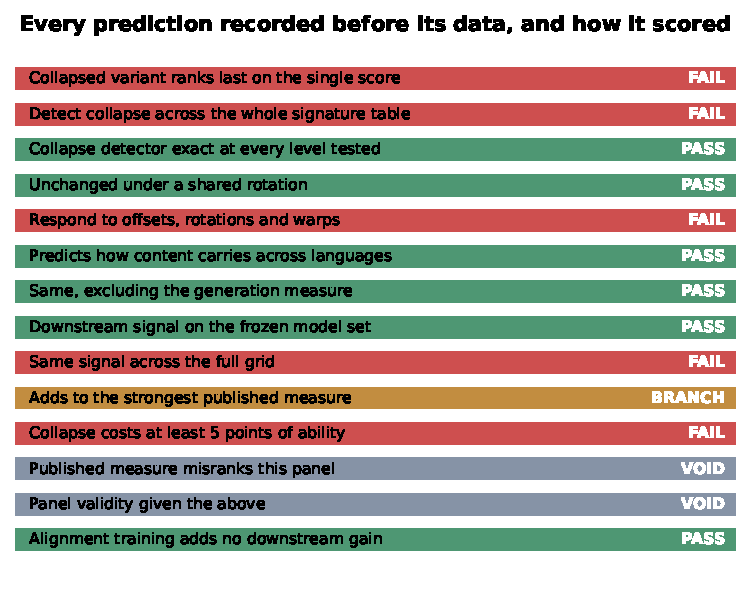
\includegraphics[width=.58\linewidth]{fig4_prediction_ledger.pdf}
\caption{Every recorded prediction and how it scored.}
\label{fig:ledger}
\end{figure}

\section{What was found}
\begin{enumerate}[label=\textbf{\arabic*.}]
\item \textbf{A share cannot see a proportional loss.} The variant
trained on the word level alignment objective lost about 95 percent of
its meaning structure at the measurement layer and posted the best LFS
score in the study; MEXA ranked it third of 25. LFS is meaning
structure against language structure, and shrinking both together
leaves the share where it was. In synthetic form the share moves less
than a millionth while meaning structure falls 99 percent. Any scale
invariant ratio inherits this. The concept variance reading, by
contrast, returns the injected magnitude exactly, to within 0.01.

\item \textbf{That damage cost the model nothing downstream.} The
degraded variant scores 0.395 on the 40 language exam against 0.390 for
the untouched control, in every seed. The variants that did lose
ability, by roughly six points, are the ones whose geometry looks
clean. Figure~\ref{fig:a5}. Representational damage and capability
damage are separable, which was not the working assumption.

\item \textbf{The mapping between languages is linear in most models,
and the exceptions are concentrated.} Across 1{,}792 model and language
pairs the fitted map is linear or simpler in 74 percent of cases, and
linear exactly in 60 percent. The nonlinear cases are not spread
thinly: three models (Falcon3-7B, OLMo-2-1B, OLMo-2-7B) carry 80
percent of them, and across the other eleven models only 6.5 percent of
languages need a nonlinear map.

\item \textbf{Each reading is worth something different.}
Figure~\ref{fig:matrix}. Meaning against language tracks how well a
model carries content across languages at 0.76; sentence matching
tracks downstream exams at 0.24 to 0.31, level with the strongest
published measure; behaviour in the weakest aligned languages tracks
which variants lost ability at 0.51, and is the only reading that does.
No reading wins twice, which is why they are reported side by side.

\item \textbf{A measure built on generation can run backwards.} A
transfer measure taken from the generation harness \emph{rises} under
mild representational damage and falls only under total destruction of
the correspondence between languages --- confirmed in trained variants,
in dose controlled synthetic worlds, and across models. Measures that
work by intervening on representations can reward the very damage they
are meant to detect.

\item \textbf{The evidence in a language panel is thinner than its
size.} Correlations across languages are so mutually dependent that a
panel of 69 languages carries the independent evidence of roughly two.
This bounds what any measure in this area can claim from per language
correlations, including these.
\end{enumerate}

\begin{figure}[t!]\centering
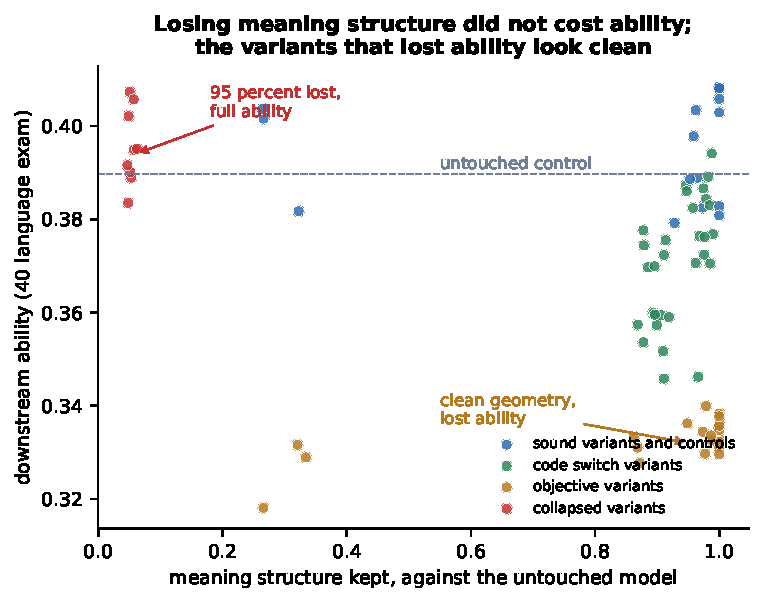
\includegraphics[width=.55\linewidth]{fig2_collapse_benign.pdf}
\caption{75 scored checkpoints. Concept preservation on the horizontal
axis, downstream ability on the vertical.}
\label{fig:a5}
\end{figure}

\section{What RMFS reports}
Four readings per language, computed from 300 parallel sentences in 41
languages at one layer, roughly four GPU minutes per model:
\begin{itemize}
\item \textbf{Meaning against language} --- the share of systematic
structure that encodes concepts rather than language identity. LFS's
original measurement, kept intact.
\item \textbf{Sentence matching} --- how reliably the model matches
sentences to their English parallels.
\item \textbf{Weakest aligned languages} --- behaviour in the poorest
aligned tail, where training damage appears first.
\item \textbf{Collapse flag} --- concept variance against a reference
checkpoint, for training settings. It detects the loss exactly and
makes no claim about ability, per finding 2.
\end{itemize}
Each reading becomes a percentile against a frozen reference grid of 14
models and the four are averaged, giving a 0--100 score per language,
with the model score as the median across languages. A score of 74
means better than 74 percent of the reference models. The ordering
falls out with no tuning: Qwen3-8B 90.5, 4B 85.7, 1.7B 73.8;
Salamandra-7B 69.0; OLMo-2-1B 28.6.

The 0.76 above is stable when whole language families are resampled
rather than languages (0.60 to 0.89) and rests on four models in that
comparison, giving 0.12 to 0.84 when models are treated as the unit.

\begin{figure}[t!]\centering
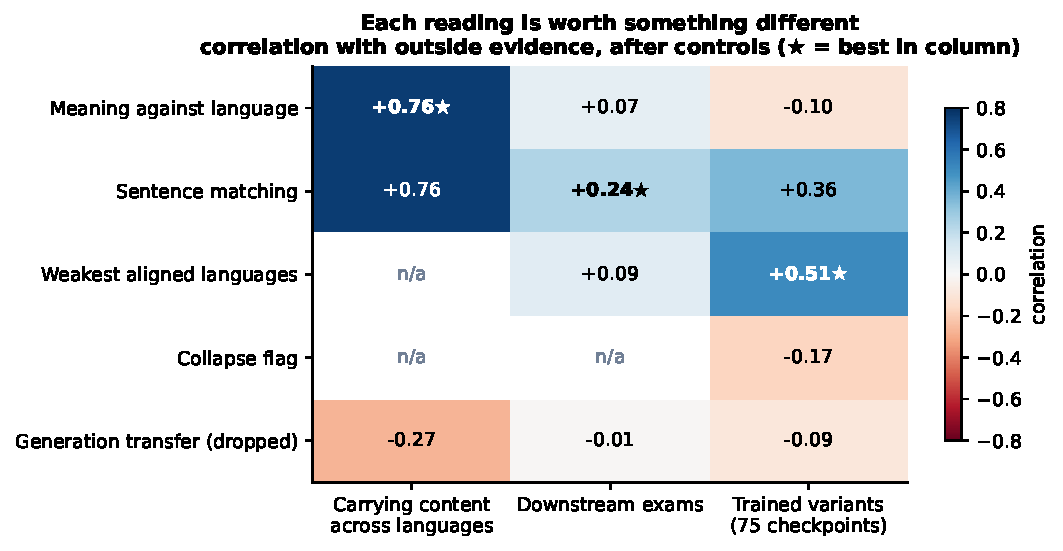
\includegraphics[width=.66\linewidth]{fig1_validity_matrix.pdf}
\caption{Each reading against each kind of outside evidence.}
\label{fig:matrix}
\end{figure}

\section{Against Aim 1's questions}
\begin{center}\small
\begin{tabular}{p{0.28\linewidth}p{0.64\linewidth}}
\toprule
\textbf{Sub aim} & \textbf{What the study provides}\\
\midrule
\textbf{3.1.1} How strong is the language component; is the mapping
just linear or more complex? &
The split between meaning and language is quantified across 14 models,
and the mapping is linear or simpler in 74 percent of model and
language pairs, with the nonlinear cases concentrated in three models
(finding 3). Both as distributions rather than single cases.\\
\addlinespace
\textbf{3.1.2} Re-visiting the logit lens &
Covered in the earlier phase (lens validity, English hub inflation);
carried as context.\\
\addlinespace
\textbf{3.1.3} Cross lingual transfer in generation &
The harness is built and validated: control patches reproduce the
reference exactly. It supplies one of the three kinds of outside
evidence used here, and produced finding 5.\\
\addlinespace
\textbf{3.1.4} Intrinsic metrics that correlate strongly with extrinsic
metrics &
Correlations are measured against three kinds of outside evidence with
the controls this area usually omits, and the same analysis quantifies
how much independent evidence a language panel carries (finding 6).\\
\bottomrule
\end{tabular}
\end{center}

\end{document}
